\chapter{Paper III:\@
  Overreact, an in silico lab:
  \linebreak automative quantum chemical microkinetic simulations
  for complex chemical reactions
 }%
\label{ch:paper3}

\fullcite{Schneider2022}

\overreact is a software package for microkinetic modelling using data from
first-principles quantum chemical
calculations~\cite{Schneider2022,overreact2021zenodo}.
It is an improvement on a first attempt to build a
chemical chemical kinetics simulator that uses first-principles quantum
chemical calculations~\cite{pyrrole2019zenodo} (for a list of other software
contributions that have taken place during the course of the PhD, see~\cref{ch:all-works}).
Lessons learned from this first iteration, as well as the methodology
underlying \overreact, can be found in~\cref{sec:overreact-methods}.

The methology was developed such that as much as possible of the physics of the problem could be included,
while still making the whole process manageable from the computational point of view.
This means choosing the use of classical transition state theory,
whose requirement of having transition state structures is attainable
using simply available computational chemistry packages of today, in contrast to other theories
such as variational transition state theory.
Although limiting, this way of doing things is accurate to a wide variety of chemical phenomena.
% TODO: CITATION FOR THE PHRASE ABOVE!

The literature is well-stablished in most of this regard.
For instance, CITE SUCH AND SUCH, theories of transition state, etc.
RRKM, Marcus theory, VTST, etc.
On other aspects, such as solvation entropy, it is actually divided CITE.\@

Regarding the emergent need for mechanistic elucidation, the research shows promissing
results in terms of doing semiautomatic hypothesis test in terms of which reactions are feasible
in a given context.
As far as we known, this is the first system that is able to produce kinetic reaction profiles
automatically from simple computational chemistry outputs and still take into account most of the physics of the problem.

% TODO: get that from the paper!
But many contributions came earlier, for instance SUCH AS SUCH.\@
Polyrate, EyringPy, MKMCXX, etc.
CITE Emílio Martínez?

It is important to do this investigation, as the demand has considerably increased throughout the years.
One can not expect to produce excellent catalytic processes without knowning how they work,
especially if there is need to \emph{systematically} and \emph{consistently} design them for various applications.
This is extremelly important in today's economy and ongoing climate crisis.

Relatedly, health applications are of utmost importance, as the world's population gets steadily older.
In this respect, cancer therapies are very important as well.

Allowing rapid rational design and investigation in those areas where understanding how reactions work is important
is a crucial effort of this work.

We aimed towards making it extremelly easy for computational discoveries in the elucidation of reaction mechanisms
to be compared with experimental data.
In this scope, one restrained the set of approachable systems to ones
being specifically investigable with today's availability of computational chemistry packages.
Although reasonably general, the method does not cover surface reactions,
some condensed state effects such as solvation entropy,
pressure-dependent reactions,
very fast reactions,
diffusion-controlled reactions,
reactions that transit between potential energy surfaces such as photochemical ones, and more.
Fully covered are room-temperature reactions in gas and solvated phases in the infinite dilution approximation.

A variety of methods were employed.
We get energies from computational chemistry packages,
together with vibrational frequencies.
Together with the molecular structure,
one is able to calculate the molecular partition function for such systems.
This allows one to calculate Gibbs' free energies and, together with reaction hypotheses,
activation free energies for such reactions.
This, together with tunneling approximations, one is able to produce accurate reaction rate constants.
% TODO: things missing for above: symmetries, etc., Grimme's stuff, etc.

% TODO:
% \section{Background and motivation}
% PRESENTATION OF THE WORK.\@
% DESCRIPTION OF THE WORK.\@
% OBJECTIVES OF THE WORK.\@
% INTERPRETATION AND MEANING OF THE WORK.\@
% MAIN FINDINGS.\@
% RESULTS IN RELATION TO THE RESEARCH QUESTIONS.\@

% TODO:
% Mecanismos foram validados com base na concordância relativa aos respectivos resultados experimentais~\cite{Kirby_1972,Jung_2005}.
% A termoquímica relevante foi calculada à condição de temperatura e pressão ambientes (298.15~K e 1~atm).
% Determinações de \emph{pKa} dos compostos estudados também foram realizadas com
% relação ao ácido acético, de acordo com o esquema de
% \citeauthor{Ding_2009}~\cite{Ding_2009} (\cref{sec:pka}).

% TODO:
% Cálculos foram realizados com o programa Gaussian~09C.01~\cite{g09} e com o funcional da densidade
% % PBE0~\cite{Perdew_1996,Perdew_1997,Ernzerhof_1999,Adamo_1999}
% \emph{wB97XD}~\cite{Chai_2008a,Chai_2008b} (\cref{sec:funcionais}), que foi
% utilizado em conjunto com funções de base de Pople de qualidade triplo-$\zeta$
% com funções difusas e polarizações em todos os átomos
% (\emph{6--311++G**}~\cite{Ditchfield_1971,Hehre_1972,Hariharan_1973,Hariharan_1974,Gordon_1980,Francl_1982,Clark_1983,Frisch_1984,Binning_1990,Blaudeau_1997,Rassolov_1998,Rassolov_2001},~\cref{sec:basis-functions}).
% Todos os cálculos levaram em consideração efeitos de solvatação aquosa através
% do uso do \emph{SMD}, desenvolvido por \citeauthor{Marenich_2009} (\cref{sec:implicit-solvation}).
% De forma a se investigar o efeito da geometria do estado fundamental, uma
% análise conformacional dos compostos foi empregada, usando o programa Open
% Babel 2.4.1~\cite{O_Boyle_2011} com o \emph{PM7} (MOPAC2016~\cite{MOPAC},~\cref{sec:conformational-analysis}).

% TODO:
% Estruturas eletrônicas dos compostos serão estudadas à luz dos \emph{NBO}
% (\cref{sec:nbos}).

% , em particular para se correlacionar o efeito cinético da substituição
% \begin{enumerate*}[label=(\roman*)]
%   \item com eventuais flutuações de hibridização dos carbonos da ponte~\cite{Bent_1961} e
%   \item com a magnitude da repulsão estérica entre substituintes e grupos reativos.
% \end{enumerate*}

% Para tanto será utilizado o programa NBO~5.9~\cite{NBO5.9} acoplado com o programa Gaussian~09C.01~\cite{g09}.

\section{Paper}

The publication can be read in full next.

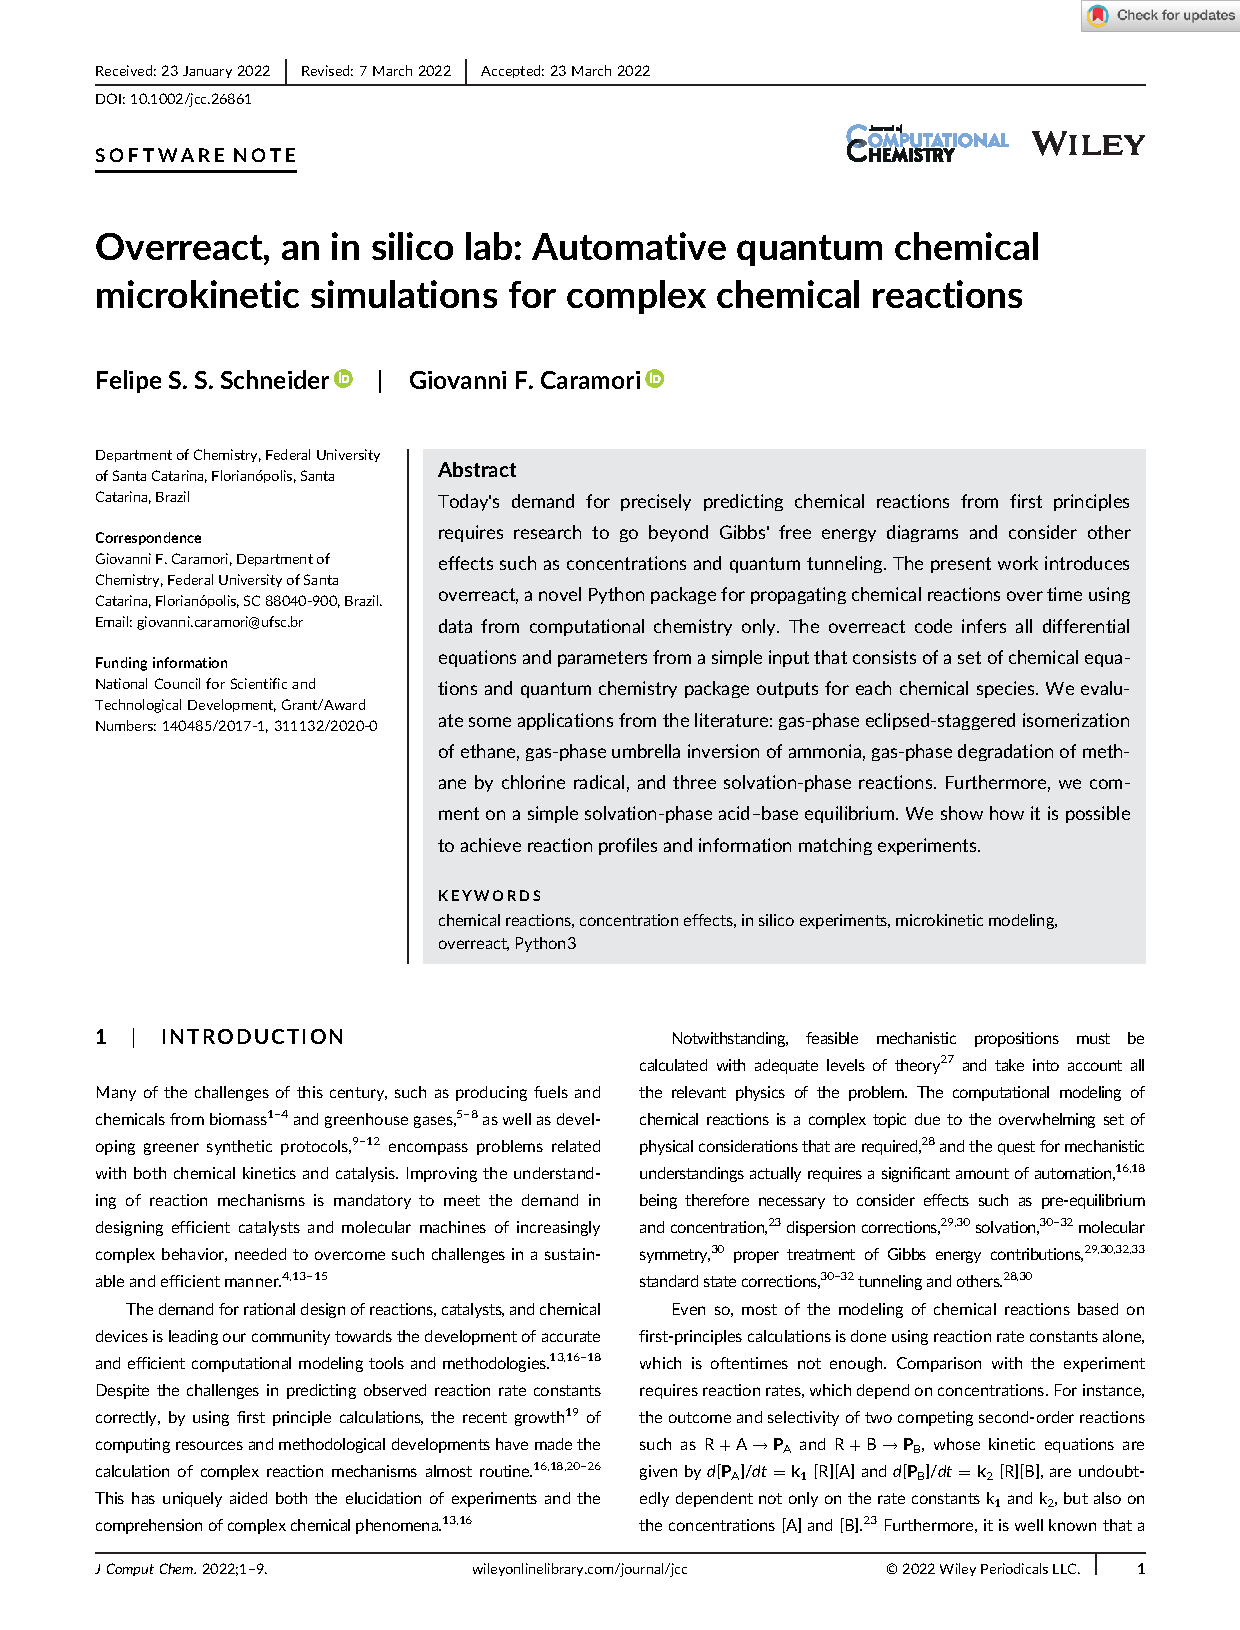
\includepdf[pages=-]{pubs/schneider2022-paper3.pdf}
